\chapter{神经网络处理器编译器验证思路}

在阐明验证思路之前,我们应首先来熟悉一下神经网络处理器的软件构架, 如图\autoref{fig:Software stock}所示,神经网络处理器的软件部分自上而下主要分成如下几个层次:

1.User Program。上层应用。即程序员基于编程框架,定义的特定的神经网络结构来实现特定的神经网络功能。

2.Framework。编程框架,相当于连接的桥梁。例如(Caffe、TensorFlow),为用户提供神经网络基本操作,减轻程序员的编程负担,是一种编程工具。

3.runtime library,库是一个屏蔽掉底层硬件,编译器、启动程序的具体信息,对上层编程框架提供神经网络原子(即神经网络的某一层,这是神经网络最基本的组成单元)操作的编程接口的系统软件。

4.driver、compile:编译器:将上层的库传来的指令描述符按照神经网络处理器的指令集翻译成能接受的机器指令。驱动:对上层库提供调用底层硬件最基本的操作支持,例如读取数据、启动关闭、读取寄存器等。

5.hardware 硬件:即神经网络处理器(DaDianNao)
\begin{figure}[!htbp]
\centering
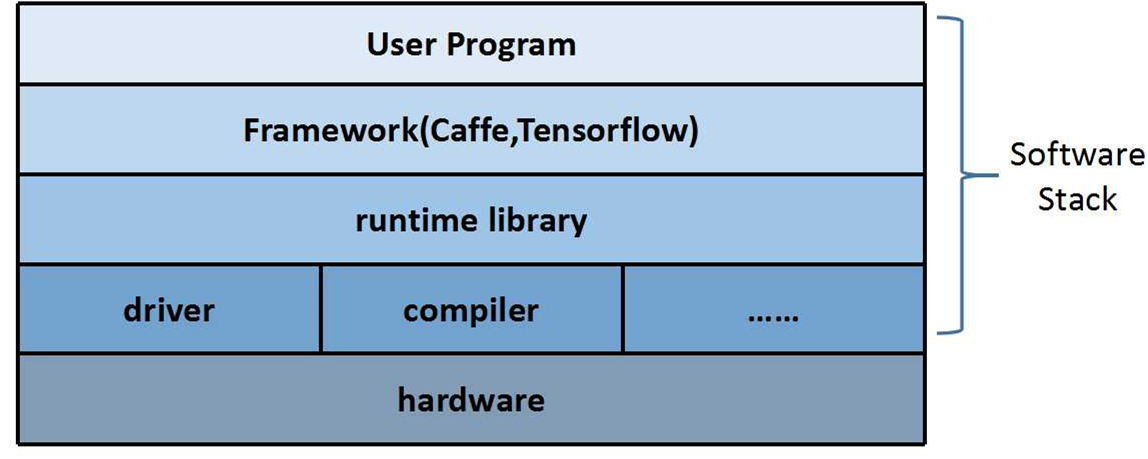
\includegraphics[width=12cm]{Software_stock.jpg}
\caption{神经网络处理器的软件架构}
\label{fig:Software stock}
\end{figure}

验证需要对变量进行控制,由于我们需要验证的是神经网络处理器的编译器,因此主要关注的是runtime library以及compiler的正确性。

prototxt -proto-caffe重载,生成随机网络,运行两次caffe分别获得ipu结果和cpu结果,对比结果是否正确,达到验证目的。

要运行caffe,首先需要先创建一个模型(model),caffe里自带了不少常用的神经网络模型,而一个模型由多个层(layer)构成,每一个层又存在着许多参数,而每一个层的参数都定义在caffe.proto这个文件内,因此,想要生成一个可以用于验证的模型,我们必须首先生成一个符合参数定义的prototxt。

\section{protext的生成}
我们自己编写了一套随机网络生成器,通过这个随机网络生成器,我们可以根据用户的需求,生成结构随机,参数随机且具有正确合理的连接方式的神经网络。同时,这个生成器也可以根据用户需求,生成包含有指定层序列、甚至是结构固定的网络。关于随机网络生成器的细节将在第三章详细概述。
\section{caffe\underline{ }model的创建}
caffe
\section{caffe重载}

\section{caffe运行ipu的过程}
Cpu 准备数据和指令,拷贝到ipu ,ipu 执行,cpu 读结果。

在我们的库(DLPlib)里,有两个主要的数据结构,张量(tensor)与滤波器(filter),这是来自于神经网络的概念。其中张量是用来描述输入和输出数据,在许多流行框架(例如Caffe以及Tensorflow),神经元和突出权重被封装在张量结构,但在我们的库中,只有神经元被表示为张量,而突触权重被封装在层中。在我们的库中,我们将张量和滤波器定义为两个独立数据的神经元和突触权重结构。对于某些操作(例如卷积和池化),一个算子以张量为形式经过一个滤波器,而后再以张量形式进行输出。
\begin{figure}[!htbp]
\centering
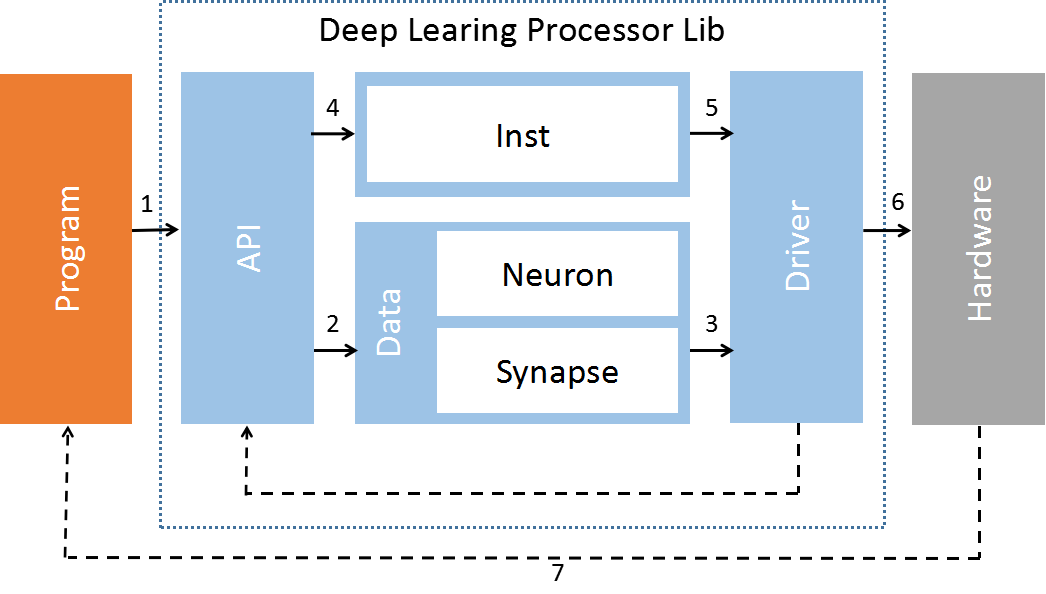
\includegraphics[width=12cm]{DLP1.png}
\caption{DLP的执行模型}
\label{fig:Software stock}
\end{figure}